\documentclass[a4paper]{article}

\usepackage[T1]{fontenc}
\usepackage[utf8]{inputenc}
\usepackage{graphicx}
\usepackage{fixme}

\usepackage[english, french]{babel}

\usepackage{hyperref}

\usepackage[sorting=ynt, maxnames=10, doi=false, url=false]{biblatex}
\addbibresource{biblio.bib}
\AtEveryBibitem{\clearfield{note}}

\usepackage{palatino}

\newcommand{\eg}{{\textit{e.g.~}}}
\newcommand{\etal}{{\textit{et al.~}}}
\newcommand{\ie}{{\textit{i.e.~}}}

\title{Vers une cognition sociale chez les robots \\ 
    {\large Programme de recherche}}

\author{Séverin Lemaignan}
\date{}

%%% Body
\begin{document}
\maketitle

La présentation de mes activités de recherche antérieures peut être comprise comme
autant de regards sur la problématique de la cognition sociale chez les robots : la
question pratique de la représentation et de la manipulation des connaissances,
la question des pré-requis sémantiques de l'interaction naturelle (verbale en
particulier), la question de la cohérence et de la faisabilité d'une
architecture cognitive intégrée pour la robotique d'interaction, la question,
aussi, de l'évaluation de l'engagement homme-robot sur le long terme.

Ces différentes facettes sont les pièces d'un puzzle auquel je me propose de
travailler dans sa globalité : \textbf{comment comprendre l'idée de \emph{cognition
sociale} chez le robot, comment la construire, comment l'évaluer ?}

Ce projet s'articule en plusieurs axes, que j'expose plus en détail ci-après.
La première question que je souhaite poser est celle-ci : Que nous enseignent
les sciences cognitives \emph{humaines} en terme de compétences cognitives
nécessaires à l'interaction entre agents et en terme d'évaluation de ces
compétences ? Une synthèse des travaux existants en sciences humaines et
neuro-sciences cognitives, et l'important travail d'adaptation à la robotique
qui en découle, apparaissent aujourd'hui incontournables pour progresser sur les
questions d'interaction sociale entre hommes et robots.

La question théorique sous-jacente est celle de la compréhension, de la
définition et de l'application de l'idée de cognition sociale en robotique. Je
souhaite donner corps à cette problématique, aujourd'hui floue car
multi-factorielle, en re-pensant l'existant (les (neuro-)sciences cognitives, donc,
mais aussi les architectures cognitives telle qu'on les connait en intelligence
artificielle) dans le cadre de la robotique sociale, avec ses dimensions
particulières (relations interpersonnelles, incarnation, sous-spécification,
dynamique). Il s'agit non seulement de construire l'idée de cognition sociale
chez le robot, mais aussi de l'envisager de manière concrète, en terme
d'implémentation sur des robots.

Un aspect saillant de cette question, et dont je propose de faire un autre de
mes axes de recherche, est la question de la \emph{représentation} de
l'environnement spatial, temporel, social et contextuel du robot. La littérature
s'intéresse essentiellement aux deux premiers points. Il me semble que les deux
derniers sont des objets encore peu étudiés et pourtant essentiels pour une
prise de décision autonome et complexe en interaction homme-robot.

Enfin, je souhaite inscrire ce programme de recherche dans une perspective
expérimentale forte. La menée systématique d'expériences d'interaction en
milieux écologiquement valides reste rare et sujette à des faiblesses
méthodologiques. En m'appuyant sur l'expérience que j'ai acquise en
post-doctorat, je souhaite en particulier travailler à la mise en place d'un
référentiel expérimental pour l'évaluation cognitive des robots, qui serait
aisément reproductible dont la méthodologie serait rigoureusement validée.

Ce projet de programme de recherche mêle étroitement robots et humains. Bien que
mise en avant de manière répétée dans les orientations scientifiques européennes
(voir par exemple la place qu'y consacre l'agenda Horizon2020 dans la section
\emph{Future and Emerging Technologies}), la robotique cognitive d'interaction
est relativement peu représentée dans le paysage scientifique français. Au sein
du CNRS, les trois principaux laboratoires travaillant sur cette thématique sont
l'\emph{Institut des Systèmes Intelligents et de Robotique} (ISIR) à Paris, le
\emph{Laboratoire d'Analyse et d'Architecture des Systèmes} (LAAS) à Toulouse,
et le \emph{Robot Cognition Laboratory} (RLC) à Lyon (unité mixte INSERM). Le
LAAS et le RLC sont des laboratoires avec lesquels j'ai déjà travaillé, et qui
seraient tout à fait adaptés pour y développer mes thèmes de recherche ; je
souhaiterais cependant, en premier choix, rejoindre l'ISIR : ce laboratoire a
une expertise reconnue aussi bien en cognition artificielle (avec de nombreuses
collaborations interdisciplinaires), que sur les questions d'interaction
(notamment au niveau du traitement des signaux sociaux). L'ISIR a récemment
acquis un robot PR2, prenant ainsi la direction de recherches sur des
architectures décisionnelles intégrées. Mon expérience antérieure avec ce type
d'architecture et le projet que je propose ici s'inscrivent naturellement dans
cette dynamique.

\subsection*{Axe 1 -- Définir la cognition sociale chez le robot}

Comme je l'ai présenté dans~\cite{lemaignan2014human}, si la robotique
cognitive, qui hérite à ce titre de la psychologie cognitive, s'intéresse aux
processus mentaux comme l'\emph{attention}, l'utilisation du \emph{langage}, la
\emph{mémoire} ou les processus de \emph{prise de décision}, la cognition
sociale y ajoute les aspects lié à la prise en compte des interactions avec
d'autres agents : \emph{représentation des croyances}, \emph{prise de
perspective}, \emph{action conjointe}, et tous les aspects liés à la
\emph{communication}.

L'une des difficultés importantes à laquelle la communauté fait face est
l'absence de référentiel permettant d'évaluer, et donc de comparer et de mesurer
les progrès des capacités cognitives des robots.  Cela tient à deux raisons
principales : d'une part, le périmètre exact de ce qu'on appelle la robotique
cognitive est relativement mal défini, ce qui rend difficile la création d'une
mesure synthétique des capacités cognitives ; d'autre part, la plupart des
outils d'évaluation à notre disposition viennent de l'étude de la cognition
humaine, et sont concrètement souvent difficile à appliquer aux robots car la
hiérarchie des compétences cognitives chez les robots est différente de celle de
l'homme : les compétences langagières, par exemple, sont difficilement
comparable. La production verbale, essentiellement traitée par la synthèse
vocale, est considérée pour un robot comme un problème moins difficile que la
compréhension orale (qui requiert, outre la reconnaissance vocale, une analyse
syntaxique et sémantique généralement difficile). Or les tests de langage que
l'on rencontre en psychologie cognitive vont typiquement se focaliser sur la
capacité à parler, en faisant l'hypothèse que l'enfant comprend ce qu'on lui dit.

De fait, la communauté robotique s'appuie aujourd'hui essentiellement sur des
évaluations qualitatives. Langley~\etal\cite{Langley2006} suggère ainsi cinq
dimensions d'évaluation : la \emph{généralité} du système (peut-il s'adapter à
une nouvelle tâche?), la \emph{rationalité} ou pertinence des
inférences/raisonnements/décisions que le système prend, la \emph{réactivité} et
la \emph{persistance} qui évalue si le comportement du système est approprié en
cas de changements non-anticipés, la capacité du système à \emph{améliorer sa
performance} comme fonction des connaissances supplémentaires qu'on lui fournit,
et enfin, \emph{l'autonomie} du système. Ces dimensions sont cependant
générales, et peu opérationnelles.

Un certain nombre d'outils issus de la psychologie cognitive ont déjà été
explorés de manière concrète sur des robots, comme les expériences de fausses
croyances (\emph{False Beliefs}~\cite{Leslie2000}), liées à la théorie de
l'esprit~\cite{Breazeal2006, warnier2012when, trafton2013act}, ou encore le
\emph{Token test}~\cite{DiSimoni1978} pour l'évaluation de certaines compétences
linguistiques~\cite{Mavridis2006}. Ces expériences ont montré qu'il était
possible et utile de ré-utiliser en les adaptant des tests de psychologie
cognitive en robotique.

D'autres recherches tentent de s'appuyer plus largement sur des expériences de
psychologie développementale, comme celles menées dans le cadre du projet
européen CHRIS, avec une équipe pluridisciplinaire incluant, outre des
laboratoires de robotique, l'INSERM (équipe de P.F. Dominey) et le Max Planck
Institute for Evolutionary Anthropology (équipe de Michael Tomasello), et
auxquelles j'ai participé~\cite{Lallee2010b}.

Elles restent cependant ponctuelles, et un travail plus
systématique et plus global reste à faire. D'autant plus que, comme l'ont
récemment souligné Zhang~\etal\cite{zhang2013evaluation}, les environnements et
métriques existants pour l'évaluation des performances cognitives des robots se
focalisent pour la plupart sur des capacités physiques, et ne requièrent pas de
capacités avancées de représentation et manipulation de connaissance, sans même
parler de compétences cognitives \emph{sociales}.

%Eux-même proposent leur une métrique basée sur la mesure du \emph{Fitness to
%Ideal Model} (FIM) d'un comportement, qu'ils corrèlent à la \emph{longueur de
%description} (DLen) de la commande qui a déclenchée le comportement. L'hypothèse
%étant que, pour un comportement donné, plus le robot a des capacités cognitives
%avancées, plus courte (c'est à dire, sous-spécifiée) pourra être la commande, le
%robot inférant le reste. Cette piste est intéressante, et est à mettre en
%relation avec d'autres approches issues des sciences cognitives humaines.

Mon objectif est ici de rechercher et de construire un référentiel rigoureux et
opérationnel pour l'évaluation des compétences cognitives des robots, en
s'intéressant à la fois à l'évaluation de chaque capacité cognitive
indépendante, et à la fois à des métriques globales de l'activité cognitive du
robot (dans~\cite{lemaignan2013explicit}, je propose une piste à explorer à ce
sujet en définissant la notion de \emph{charge cognitive} du robot en terme de
flux de connaissances échangés). Ce référentiel, s'il doit rester opérationnel,
peut aussi être ambitieux, et intégrer par exemple des techniques récentes
d'imagerie cérébrale pour l'étude de l'interaction~\cite{dumas2010inter}.

Ce premier axe de recherche propose donc de réaliser d'abord la synthèse des
travaux en sciences cognitives aussi bien en terme de construction de
l'interaction que d'évaluation des compétences cognitives, puis ensuite
d'aligner ces résultats avec les spécificités de la robotique. Les objectifs
sont d'une part une définition effective du concept de cognition sociale en
robotique, et d'autre part la conception et l'implémentation d'un référentiel
expérimental d'évaluation des compétences cognitives des robots d'interaction.

\subsection*{Axe 2 -- Représentation du monde et cognition}

\begin{figure}
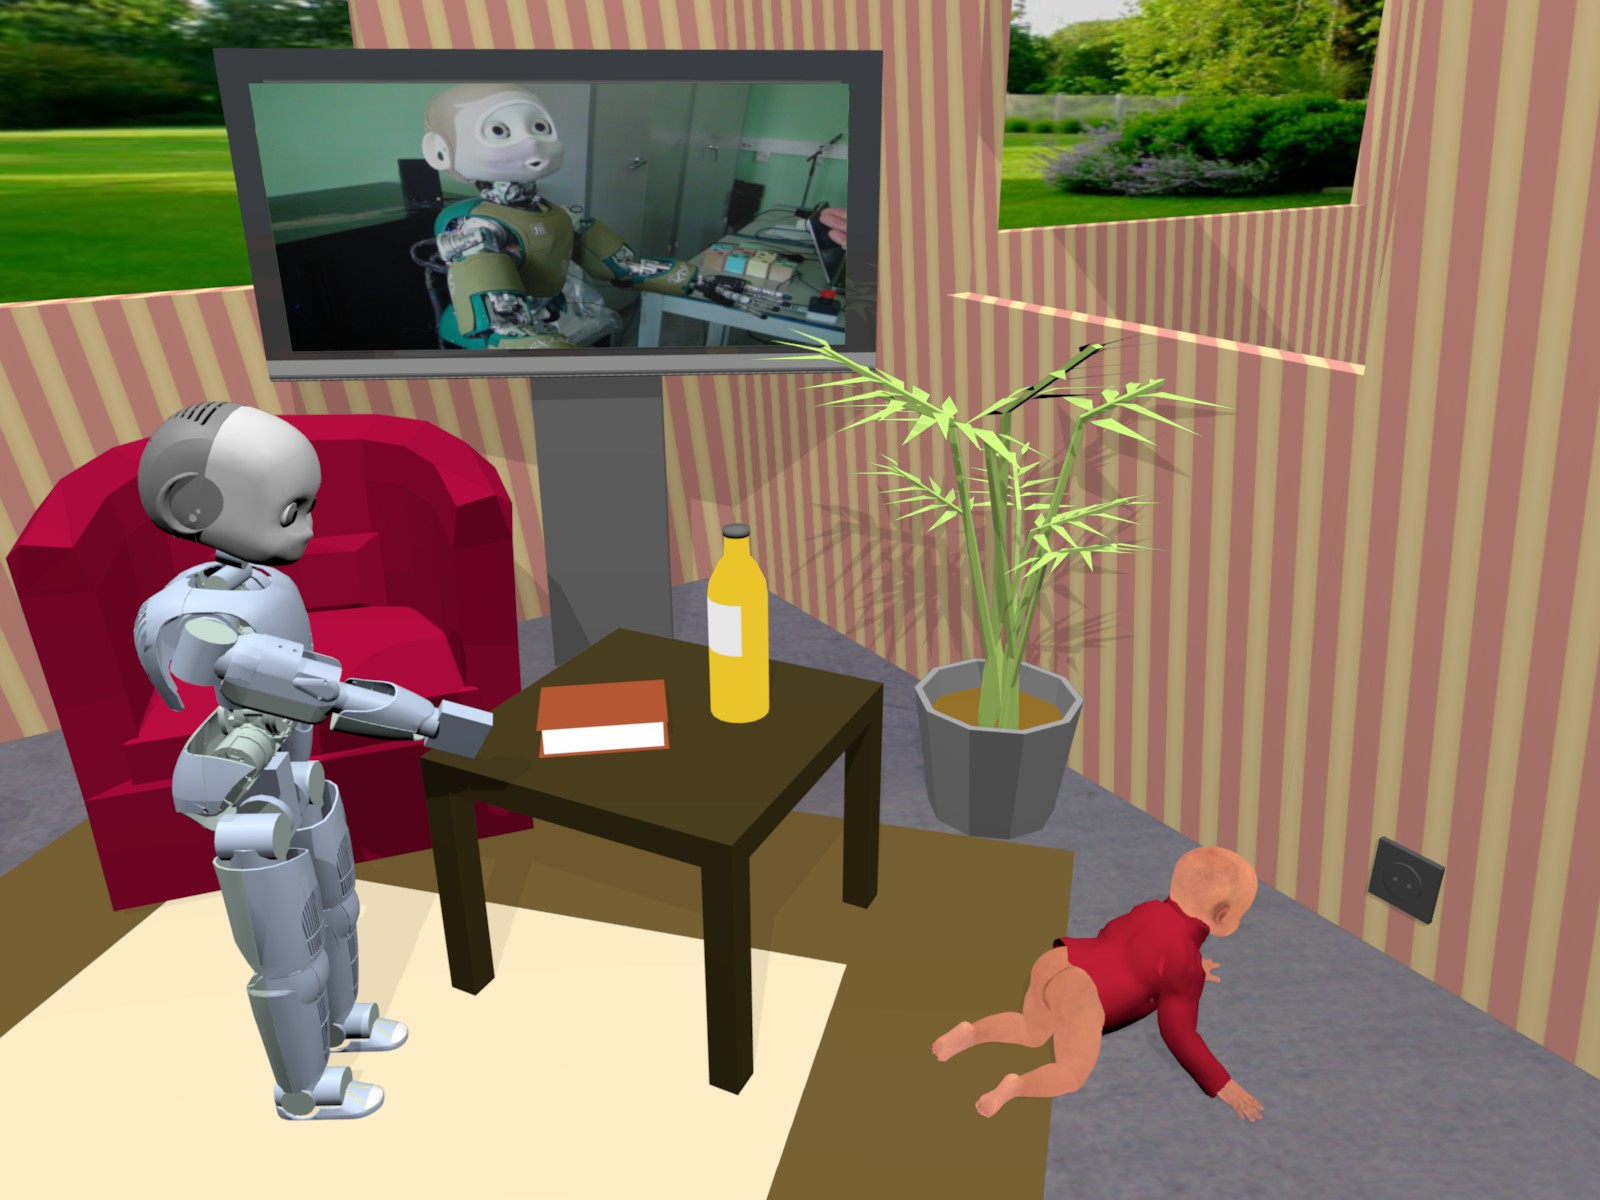
\includegraphics[width=\textwidth]{figs/robots_home_baby_socket.jpg}
\caption{Pour comprendre cette situation et anticiper le danger, il est
    nécessaire de construire une représentation \emph{unifiée} de
    l'environnement, incluant modèle géométrique (l'agencement de la pièce), modèle
    symbolique (le bébé, la prise), modèle temporel prédictif (déplacement du
    bébé), modèle des affordances \emph{pour le bébé} et enfin modèle des
    croyances et intentions du bébé.}
\label{babyplug}
\end{figure}

Le travail que j'ai mené durant mon doctorat m'a amené à analyser huit systèmes
de représentation des connaissances effectivement déployés sur des robots. Un
point clé de comparaison de ces systèmes est leur approche de l'ancrage
symbolique (\emph{symbol grounding}) dans leur environnement physique, et il en
ressort que la capacité pour un robot à représenter son environnement est à la
fois la pierre angulaire de ses capacités cognitives supérieures (raisonnement,
prise de décision, communication) et un défi qui n'est pas aujourd'hui traité
dans toute son ampleur.

Les recherches actuelles sont essentiellement focalisées sur la représentation
géométrique de l'environnement du robot. La construction en ligne de
cartes sémantiques~\cite{Nuechter2008, Galindo2008,
Blodow2011} ou l'utilisation d'affordances fonctionnelles~\cite{Varadarajan2011}
sont des exemples de l'état de l'art au regard de la construction de liens
géométrique-symbolique sur l'environnement spatial du robot.

De même, le travail sur une représentation \emph{amodale} de
l'environnement~\cite{Mavridis2006}, prenant en compte les incertitudes et
permettant de représenter des entités spatiales non-vues (donc de les imaginer),
apporte plusieurs idées importantes, mais se cantonne essentiellement aux
aspects spatiaux.

La représentation de l'environnement temporel du robot a aussi fait l'objet de
recherches (avec les idées de \emph{chroniques}~\cite{Ghallab1996}, les
approches par \emph{fluents}~\cite{mosenlechner2010becoming}, ou encore les
\emph{instantanés} proposés par Mavridis~\cite{Mavridis2006}), mais la plupart
de ces travaux s'apparentent à une journalisation des événements, accompagnée
d'outils d'analyse et d'apprentissage (en général hors-ligne). Ni la possibilité
de naviguer naturellement dans les états antérieurs, ni la création et la
représentation d'états futurs hypothétiques ne sont intégrées au niveau d'une
représentation globale de l'environnement du robot.

Quant à l'intégration de la représentation d'affordances, de contextes (en
particulier, de contextes sociaux, comme dans la figure~\ref{babyplug}, où le
robot est dans un contexte du type ``veiller sur le bébé''), de modèles de
croyances et d'intentions, le travail reste largement à faire (on peut toutefois
mentionner la représentation de différentes perspectives, comme
dans~\cite{ros2010which}). Le premier de ces défis étant d'ailleurs de concevoir
une modalité de représentation pour les affordances, contextes, croyances qui
puisse être unifiée dans un modèle de l'environnement.

Cette axe de recherche, qui prend son point de départ dans mon travail de
post-doctorat au LAAS, vise à faire progresser l'état de l'art dans le domaine
de l'ancrage symbolique en proposant de concevoir et d'implémenter une
représentation unifiée de l'environnement du robot, fusionnant les modèles
continus (modèles géométrique, historique des évènements, etc.) et les modèles
symboliques (connaissances symboliques générales sur le monde, croyances des
agents, affordances, etc.). Je conçois ce modèle de l'\emph{Umwelt} du robot (le
monde \emph{perçu}, \emph{propre} du robot) comme une brique importante devant
servir de support pour le développement et l'intégration d'architectures
décisionnelles pour les robots.

\subsection*{Axe 3 -- Architectures cognitives pour l'interaction homme-robot}

L'idée de \emph{robotique cognitive} n'est pas récente (elle est mentionnée dès
le début des années 1990 par Reiter~\cite{Levesque2008}), et est déjà établie
comme un champ de recherche actif, formant le pendant des approches
développementales de la robotique. Si ce domaine n'est pas nouveau, il est cependant
traité de manière essentiellement atomique en robotique : les compétences
cognitives sont implémentées et testées indépendamment les unes des autres, et
comme le note Kurup~\cite{kurup2012what}, ce n'est que récemment que la
robotique s'intéresse aux architectures cognitives holistiques développées en
intelligence artificielle. Les travaux de Chen~\cite{Chen2010}, de
Beetz~\etal~\cite{Beetz2010}, de Trafton~\etal sur ACT-R/E~\cite{trafton2013act}
ou les recherches menées par Baxter dans le cadre du projet européen
ALIZ-E~\cite{baxter2013cognitive} en sont les principaux exemples récents.

ACT-R/E est un exemple intéressant dans la mesure où l'architecture est conçue
en premier lieu pour l'interaction homme-robot, et elle est évaluée en se
référant explicitement à la psychologie développementale. Elle illustre aussi le
chemin qui reste à parcourir dans ce domaine : bien qu'étant une architecture
cognitive globale, elle n'a été testée que sur des compétences cognitives
isolées, en laboratoire, et ignore largement les problématiques d'ancrage
symbolique (le robot raisonne sur un environnement simplifié, et les modalités
de communication sont elles aussi simples -- pas d'interaction linguistique, par
exemple).

Mais de manière générale, encore peu de travaux s'intéressent à l'étude des
architectures cognitives dans le cadre de l'interaction homme-robot. J'ai montré
durant mon doctorat qu'il était possible de construire et d'exploiter en ligne
des modèles cognitifs riches des autres agents, et d'intégrer ces modèles dans
la prise de décision~\cite{alami2011when, warnier2012when, lemaignan2014human}.
Pour autant, une traduction systématique de mécanismes de cognition sociale en
terme d'architecture décisionnelle est une question essentiellement ouverte. La
prise en compte de codes et comportements sociaux implicites (ébauchée au niveau
de la planification symbolique dans des travaux comme~\cite{Alili2009}) ou
l'analyse d'environnements particulièrement riches en terme de sémantique (comme
l'illustre la figure~\ref{babyplug}) sont des exemples des spécificités de
l'interaction homme-robot qui ont un impact important sur la conception d'une
architecture de contrôle.

Ce troisième axe de recherche vise non seulement à bâtir les ponts nécessaires
entre les approches théoriques et fondamentales des deux précédents axes d'une
part, et les applications expérimentales de cette recherche d'autre part. Il
s'agit aussi d'implémenter et d'organiser de manière formelle un nombre élevé de
mécanismes cognitifs ego- \emph{et} allocentrés en une architecture complète et pertinente, apte à être
déployée sur des robots d'interaction autonomes.

\subsection*{Programme expérimental}

Je propose de matérialiser les axes de recherche que j'ai présenté autour de
quatre objectifs expérimentaux, qui vont de la conception et de
l'implémentation d'une méthodologie expérimentale pour évaluer les compétences
cognitives des robots, au déploiement d'un robot manipulateur mobile de type
PR2 dans une famille non-experte pour une durée longue (supérieure à un mois).
Ces quatre objectifs me permettent aussi de proposer un agenda prévisionnel
pour mes premières années de recherche.

Le premier objectif consiste donc à formaliser une méthodologie expérimentale
pour l'évaluation des capacités cognitives d'un robot social. Cet outil doit
être applicable à différentes plateformes robotiques, et je souhaite l'évaluer
en croisant différentes architectures cognitives déjà existantes avec différents
robots.  Je me fixe un horizon à J+12 mois pour atteindre cet objectif, qui
pré-suppose un travail d'analyse et de synthèse des outils existants en
psychologie développementale et cognitive ainsi qu'en intelligence
artificielle.

La seconde expérience vise à démontrer l'intérêt d'une représentation unifiée de
l'environnement du robot: l'idée est de se placer dans plusieurs scénarii
d'interaction dans l'esprit de la figure~\ref{babyplug}, pour lesquels une
interprétation correcte nécessite de combiner représentations géométriques et
symboliques, d'être capable de représenter des états futurs hypothétiques, et de
reconnaitre et mobiliser un ensemble de contextes complémentaires. Je souhaite
alors évaluer la qualité et la pertinence du modèle et de l'interprétation de la
scène créés par le robot, en les comparant aux interprétations produites par des
sujets humains. La mise en place de cette expérience requiert des développements
conséquents, et je me fixe un horizon à environ J+18 mois pour une première
série d'expériences.

La troisième expérience s'intéresse à la fois au déploiement d'une architecture
cognitive pour l'interaction en autonomie, et aux facteurs cognitifs d'une
interaction de longue durée. L'objectif est de déployer des robots de type Nao avec
des schémas d'interaction restant simples (tâches du type lecture de recette ou
d'histoire pour les enfants) dans des familles non-expertes, et sur des
périodes longues (de l'ordre de 3 mois). Cela vise à acquérir et valider les
facteurs, tant humains que robotiques, qui permettent d'établir un engagement
durable.  Je souhaite échelonner plusieurs déploiements dans plusieurs familles
en parallèle, et cette expérience pourrait s'étaler de J+24 mois à J+30 mois.

Enfin, en s'appuyant sur les enseignements issus de l'expérience précédente, le
dernier objectif expérimental, plus ambitieux, consiste à déployer un robot
complexe type PR2, dans une famille, pour une durée longue, et avec un
répertoire d'interactions étendu, incluant autonomie complète, dialogue
multi-modal, manipulation conjointe. Je situe cet objectif expérimental à un
horizon J+36 mois. Au-delà du défi scientifique que cela représente (il
s'agirait d'une première internationale), cette expérience aurait probablement
un impact sociétal, et représenterait à ce titre une étape dans la recherche en
interaction homme-robot.

Ce programme expérimental vise à faire avancer significativement l'état de l'art
en ce qui concerne la robotique d'interaction. La plateforme expérimentale
proposée par l'ISIR est l'une des rares en France qui permette d'envisager
raisonnablement ce programme, et c'est aussi une des raisons pour lesquelles je
souhaite rejoindre ce laboratoire.

\subsection*{Pour conclure}

En paraphrasant McCarthy, on peut dire de ce projet de recherche qu'il s'inscrit
dans le programme (à long terme) d'une ``intelligence incarnée de niveau
humain''. Il se positionne sur la question particulière de \emph{l'intelligence
sociale} dans le contexte d'interactions entre agents artificiels physiques et
humains.

Je propose dans un premier temps de poser des bases rigoureuses, qui semblent
aujourd'hui manquer, à l'analyse et l'évaluation des performances cognitives des
robots, en particulier dans ce contexte social.

Je propose ensuite d'attaquer la question de la fusion des représentations
multiples de l'environnement du robot, parfois continues, parfois symboliques,
en un modèle unifié. Ce modèle doit de plus intégrer des dimensions nouvelles
(contextes, affordances, modèles de croyances des différents agents), et
construire ainsi des fondations solides pour les processus cognitifs supérieurs.
C'est une question de recherche aujourd'hui ouverte, qui fait appel à des
techniques de représentations hybrides qui sont à découvrir.

Sur cette base, je propose de travailler sur l'intégration de mécanismes
cognitifs multiples au sein d'une architecture logicielle pertinente pour un
robot d'interaction. C'est ici au contraire un travail de synthèse, qui
s'appuie, en le développant, sur le corpus scientifique existant, tant en
robotique qu'en intelligence artificielle (architectures cognitives), qu'en
sciences et neuro-sciences cognitives (modèles décisionnels humains).

Enfin, parce que la recherche en robotique a aussi cette spécificité d'être une
science de l'intégration technologique, je propose d'organiser mon travail de
chercheur autour d'objectifs expérimentaux ambitieux, qui puissent aussi donner
à voir et à réfléchir sur l'impact de la recherche sur la vie de tous les
citoyens.

\printbibliography

\end{document}
